% State space diagram of the bivariate dual change score model (vignette lcs).
\documentclass[tikz, border = 6pt]{standalone}
\usepackage{amsmath}
\usepackage{bm}
\usetikzlibrary{arrows.meta, positioning, calc}
\tikzset{
  lat/.style = {circle, draw, thick, minimum size = 13mm, inner sep = 0pt},
  obs/.style = {rectangle, draw, thick, minimum size = 11mm, inner sep = 1pt},
  noise/.style = {circle, draw, minimum size = 9.5mm, inner sep = 0pt},
  reg/.style = {-{Stealth[length = 2.5mm]}, thick},
  cov/.style = {{Stealth[length = 2mm]}-{Stealth[length = 2mm]}},
  var/.style = {cov, looseness = 5},
  lab/.style = {font = \footnotesize, fill = white, inner sep = 1pt},
  mat/.style = {font = \small, inner sep = 2pt, align = left},
  dots/.style = {font = \Large}
}
\begin{document}
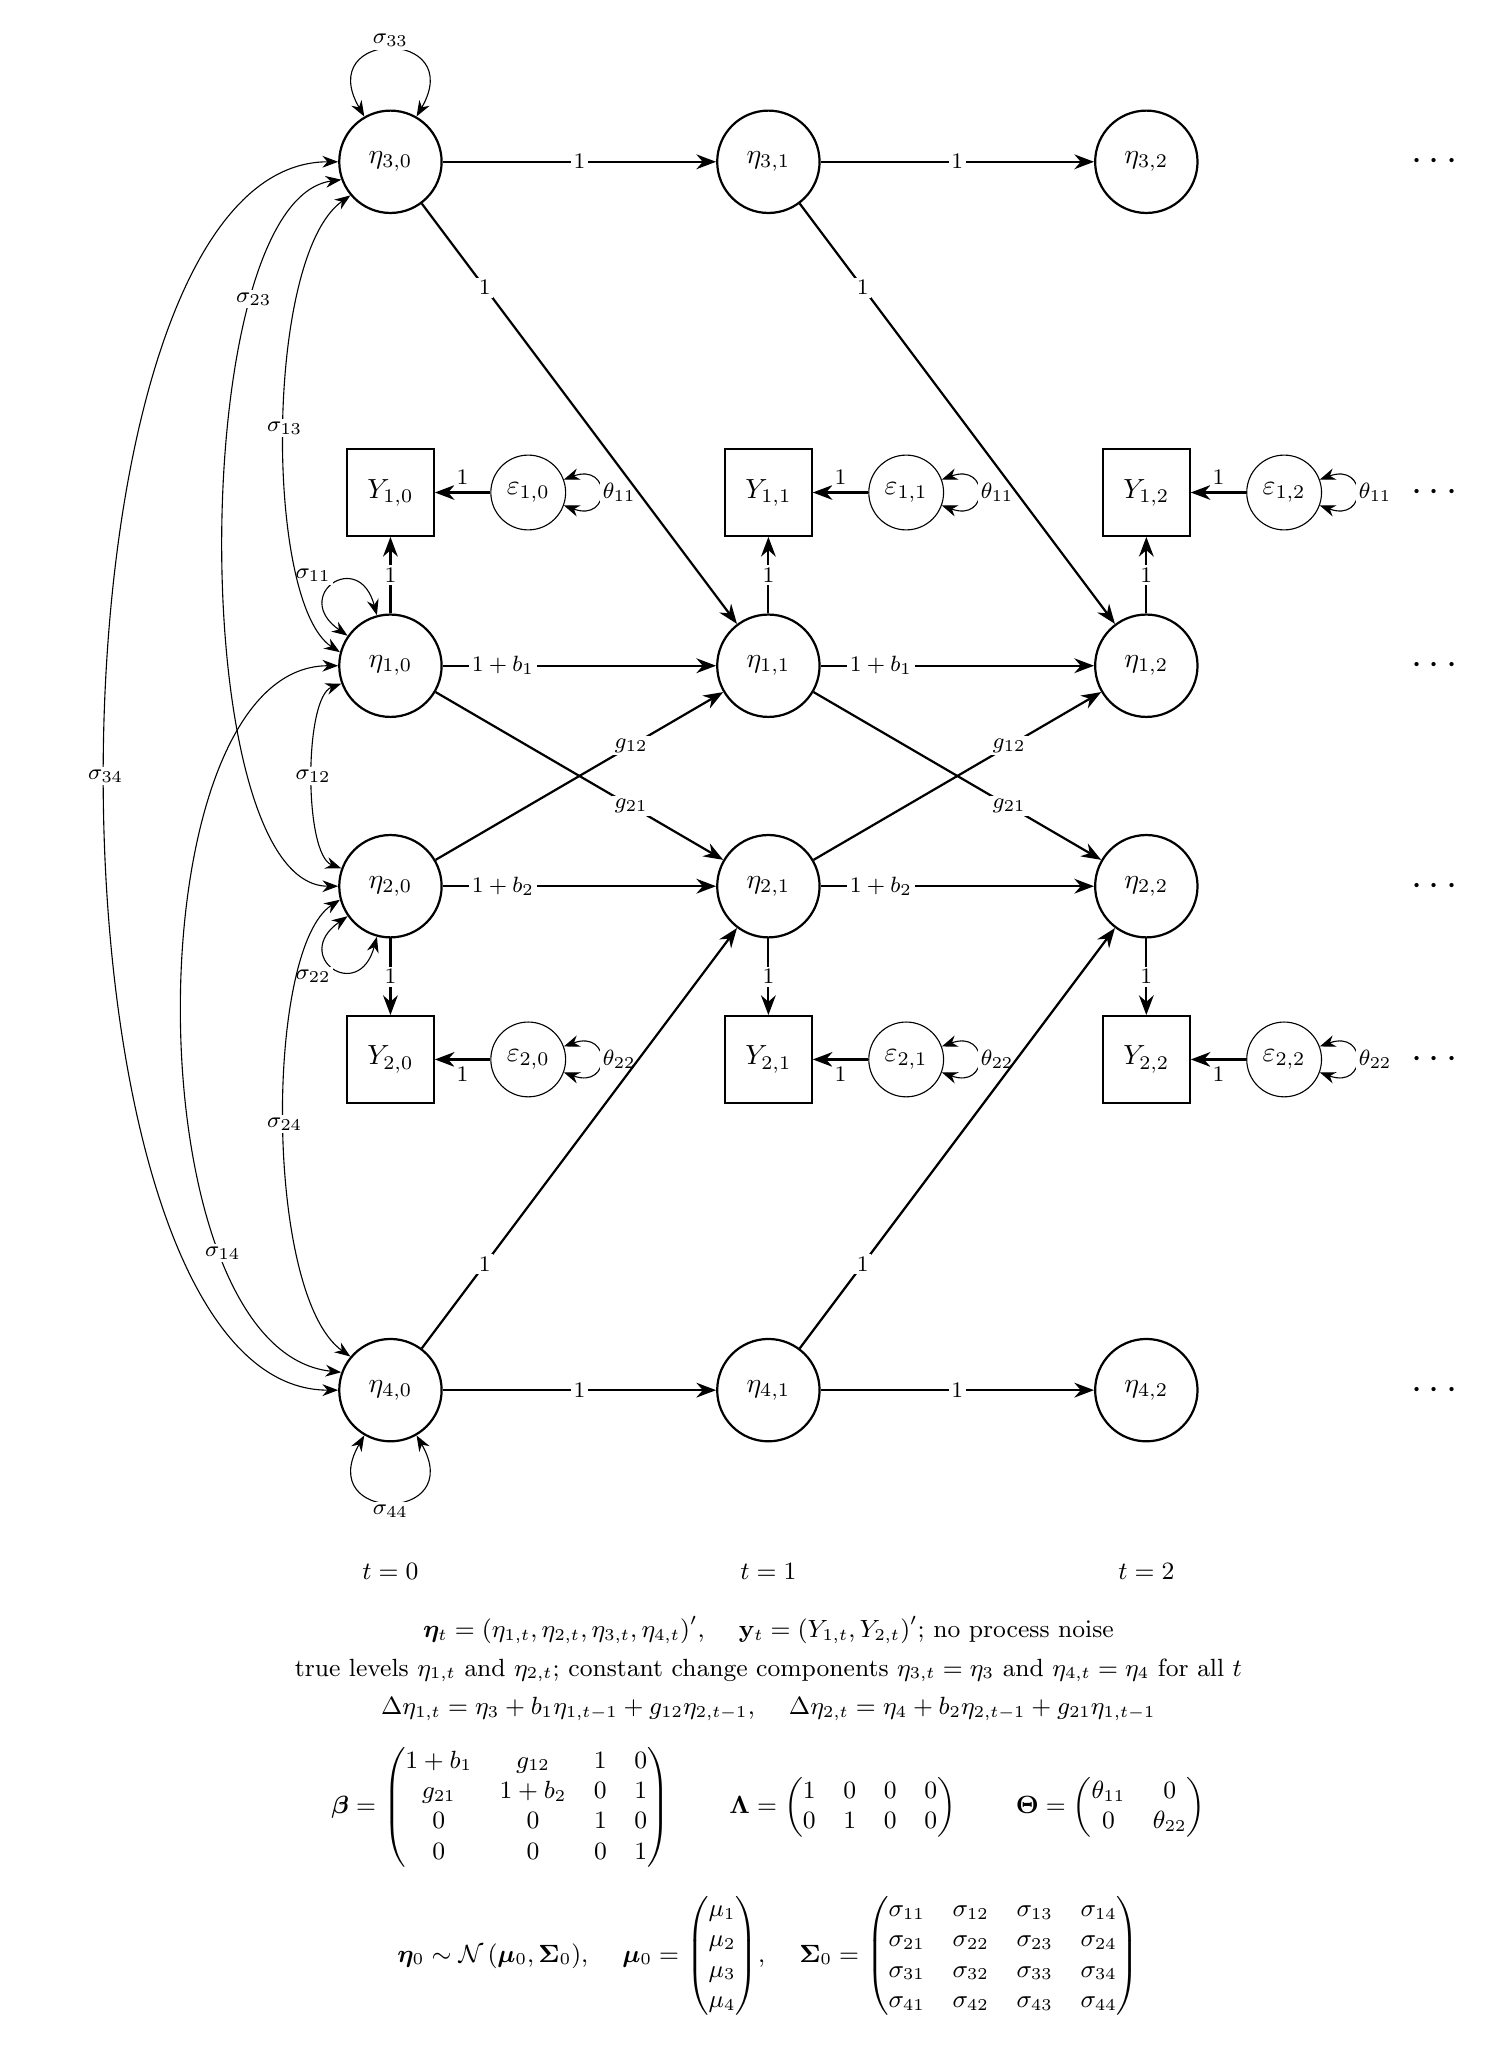
\begin{tikzpicture}
  % occasions
  \foreach \t/\x in {0/0, 1/4.8, 2/9.6} {
    \node[lat] (c\t) at (\x, 7.5) {$\eta_{3, \t}$};
    \node[obs] (p\t) at (\x, 3.3) {$Y_{1, \t}$};
    \node[lat] (a\t) at (\x, 1.1) {$\eta_{1, \t}$};
    \node[lat] (b\t) at (\x, -1.7) {$\eta_{2, \t}$};
    \node[obs] (q\t) at (\x, -3.9) {$Y_{2, \t}$};
    \node[lat] (d\t) at (\x, -8.1) {$\eta_{4, \t}$};
    \draw[reg] (a\t) -- node[lab] {1} (p\t);
    \draw[reg] (b\t) -- node[lab] {1} (q\t);
    % measurement error
    \node[noise] (u\t) at (\x + 1.75, 3.3) {$\varepsilon_{1, \t}$};
    \node[noise] (v\t) at (\x + 1.75, -3.9) {$\varepsilon_{2, \t}$};
    \draw[reg] (u\t) -- node[lab, above = 0.5mm] {1} (p\t);
    \draw[reg] (v\t) -- node[lab, below = 0.5mm] {1} (q\t);
    \draw[var] (u\t.20) to[out = 20, in = -20]
      node[lab, right] {$\theta_{11}$} (u\t.-20);
    \draw[var] (v\t.20) to[out = 20, in = -20]
      node[lab, right] {$\theta_{22}$} (v\t.-20);
    \node[font = \small] at (\x, -10.4) {$t = \t$};
  }
  % transitions
  \foreach \s/\t in {0/1, 1/2} {
    \draw[reg] (c\s) -- node[lab, pos = 0.5] {1} (c\t);
    \draw[reg] (d\s) -- node[lab, pos = 0.5] {1} (d\t);
    \draw[reg] (c\s) -- node[lab, pos = 0.2] {1} (a\t);
    \draw[reg] (d\s) -- node[lab, pos = 0.2] {1} (b\t);
    \draw[reg] (a\s) -- node[lab, pos = 0.22] {$1 + b_{1}$} (a\t);
    \draw[reg] (b\s) -- node[lab, pos = 0.22] {$1 + b_{2}$} (b\t);
    \draw[reg] (b\s) -- node[lab, pos = 0.68] {$g_{12}$} (a\t);
    \draw[reg] (a\s) -- node[lab, pos = 0.68] {$g_{21}$} (b\t);
  }
  \foreach \r in {7.5, 3.3, 1.1, -1.7, -3.9, -8.1} {
    \node[dots] at (13.3, \r) {$\cdots$};
  }
  % initial condition: variances
  \draw[var] (c0.60) to[out = 60, in = 120]
    node[lab, above] {$\sigma_{33}$} (c0.120);
  \draw[var] (d0.240) to[out = 240, in = 300]
    node[lab, below] {$\sigma_{44}$} (d0.300);
  \draw[var] (a0.105) to[out = 105, in = 145]
    node[lab, above left] {$\sigma_{11}$} (a0.145);
  \draw[var] (b0.215) to[out = 215, in = 255]
    node[lab, below left] {$\sigma_{22}$} (b0.255);
  % initial condition: covariances
  \draw[cov] (a0.200) .. controls (-1.1, 0.7) and (-1.1, -1.3) ..
    node[lab] {$\sigma_{12}$} (b0.160);
  \draw[cov] (c0.220) .. controls (-1.6, 6.3) and (-1.6, 1.9) ..
    node[lab] {$\sigma_{13}$} (a0.165);
  \draw[cov] (d0.140) .. controls (-1.6, -6.9) and (-1.6, -2.5) ..
    node[lab] {$\sigma_{24}$} (b0.195);
  \draw[cov] (c0.200) .. controls (-2.6, 7.0) and (-2.6, -1.7) ..
    node[lab, pos = 0.25] {$\sigma_{23}$} (b0.180);
  \draw[cov] (d0.160) .. controls (-3.3, -7.6) and (-3.3, 1.1) ..
    node[lab, pos = 0.25] {$\sigma_{14}$} (a0.180);
  \draw[cov] (c0.180) .. controls (-4.6, 7.5) and (-4.6, -8.1) ..
    node[lab] {$\sigma_{34}$} (d0.180);
  % matrices
  \node[mat, align = center, below] at (4.8, -10.9) {%
    $\bm{\eta}_{t} = \left( \eta_{1, t}, \eta_{2, t}, \eta_{3, t},
      \eta_{4, t} \right)^{\prime}$, \quad
    $\mathbf{y}_{t} = \left( Y_{1, t}, Y_{2, t} \right)^{\prime}$;
    no process noise \\[1mm]
    true levels $\eta_{1, t}$ and $\eta_{2, t}$; constant change components
    $\eta_{3, t} = \eta_{3}$ and $\eta_{4, t} = \eta_{4}$ for all $t$
    \\[1mm]
    $\Delta \eta_{1, t} = \eta_{3} + b_{1} \eta_{1, t - 1}
      + g_{12} \eta_{2, t - 1}$, \quad
    $\Delta \eta_{2, t} = \eta_{4} + b_{2} \eta_{2, t - 1}
      + g_{21} \eta_{1, t - 1}$ \\[3mm]
    $\bm{\beta} = \begin{pmatrix}
      1 + b_{1} & g_{12} & 1 & 0 \\ g_{21} & 1 + b_{2} & 0 & 1 \\
      0 & 0 & 1 & 0 \\ 0 & 0 & 0 & 1
    \end{pmatrix}$
    \qquad $\bm{\Lambda} = \begin{pmatrix}
      1 & 0 & 0 & 0 \\ 0 & 1 & 0 & 0
    \end{pmatrix}$
    \qquad $\bm{\Theta} = \begin{pmatrix}
      \theta_{11} & 0 \\ 0 & \theta_{22}
    \end{pmatrix}$ \\[3mm]
    $\bm{\eta}_{0} \sim \mathcal{N} \left( \bm{\mu}_{0},
      \bm{\Sigma}_{0} \right)$, \quad
    $\bm{\mu}_{0} = \begin{pmatrix}
      \mu_{1} \\ \mu_{2} \\ \mu_{3} \\ \mu_{4}
    \end{pmatrix}$, \quad
    $\bm{\Sigma}_{0} = \begin{pmatrix}
      \sigma_{11} & \sigma_{12} & \sigma_{13} & \sigma_{14} \\
      \sigma_{21} & \sigma_{22} & \sigma_{23} & \sigma_{24} \\
      \sigma_{31} & \sigma_{32} & \sigma_{33} & \sigma_{34} \\
      \sigma_{41} & \sigma_{42} & \sigma_{43} & \sigma_{44}
    \end{pmatrix}$};
\end{tikzpicture}
\end{document}